% !TeX TS-program = txs:///duck
\documentclass{standalone}
\usepackage{tikzducks}

\begin{document}
	
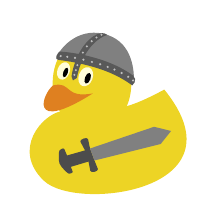
\begin{tikzpicture}
	\duck[helmet]
	\fill[gray!60!black] (0.5831,0.5821) -- (0.8112,0.6468) -- (0.7528,0.7563) .. controls (0.7367,0.7865) and (0.8427,0.8231) .. (0.8497,0.7897) -- (0.8749,0.6705) -- (0.9316,0.5183) -- (0.9744,0.4102) .. controls (0.9865,0.3796) and (0.8848,0.3549) .. (0.8784,0.3872) -- (0.8553,0.5051) -- (0.6311,0.4379) -- (0.6541,0.3774) .. controls (0.6619,0.3569) and (0.6051,0.3422) .. (0.5908,0.3589) .. controls (0.5908,0.3589) and (0.5068,0.4303) .. (0.4875,0.4797) .. controls (0.4692,0.5265) and (0.4818,0.6305) .. (0.4818,0.6305) .. controls (0.4809,0.6553) and (0.5387,0.6862) .. (0.5484,0.6634) -- cycle;
	\fill[gray] (0.8749,0.6705) -- (1.6884,0.9465) -- (1.9041,0.8933) -- (1.7728,0.7282) -- (0.9316,0.5183) -- cycle;
\end{tikzpicture}	
	
\end{document}